\documentclass[main]{subfiles}
\begin{document}

%@@@@@@@@@@@@@@@@@@@@@@@@@@@@@@
% Main Topics: graphs and TU matrices, max-flow min-cut
% Applications of Total Unimodularity - 16.11.2017
% Joe covered Weismantell in this lecture
% author: Vanessa Leite

\section{Applications of Total Unimodularity}

\paragraph{A important reminder:}
Theorem: $A \in \{0, \pm 1\}^{m \times n}$ is TU iff $\forall J \subseteq [n]$
(or $J \subseteq [m]$ because $A^T$ is also TU) $\exists$ partition $J = J_1
\cup J_2$ such that $\sum_{j \in J_1} A_{ij} - \sum_{j \in J_2} A_{ij} \in \{0,
\pm 1\}$ iff $\max \{c^T x \mid Ax \leq b\}$ has an \textbf{integral} optimal
solution for every $b \in \Z^n$, wherever an optimal solution exists, iff $A^T$
is TU.

\paragraph{Definition - Digraph}
Let $V$ be a finite set and $A \subseteq V \times V$. Then $D=(V,A)$ is a
digraph (directed graph).

\paragraph{Definition - Node-arc incidence matrix}
The node-arc incidence matrix of $D=(V,A)$ is the matrix
$M \in \{0, \pm1\}^{\abs{V} \times \abs{A}}$, where $M_{ia} = 
\left\{
  \begin{array}{ll}
    1 & \text{if } (i,j) = a \\
    -1 & \text{if } (j,i) = a \\
    0 & \text{else}
  \end{array}
\right.$

\paragraph{Definition}
Let $w \subseteq V$.\\
$\delta^+(w) = \{(i,j) \in A, i \in w, j \notin w \}$.\\
$\delta^-(w) = \{(i,j) \in A, i \notin w, j \in w \}$.\\
\subparagraph{Example:}
\begin{figure}[!h]
  \label{fig:projection}
  \centering
    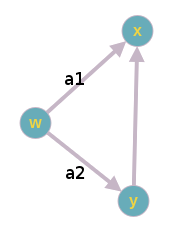
\includegraphics[width=0.3\textwidth]{imgs/graph-definition.png}
\end{figure}

$\delta^+(w) = \{a1,a2\}$.\\
$\delta^-(w) = \emptyset$.\\

\paragraph{Definition - Node-edge incidence matrix}
The node-edge incidence matrix of an undirected graph $G=(V,E)$ is
$M \in \{0,1\}^{\abs{V} \times \abs{E}}$, where $M_{ve} = 
\left\{
  \begin{array}{ll}
    1 & \text{if } e = (v,w)\\
    0 & \text{else}
  \end{array}
\right.$

\paragraph{Theorem: The following matrices are TU:}
\begin{enumerate}
\item The node-arc incidence matrix of a digraph
\item The node-edge incidence matrix of a bipartite undirected graph
\item An interval matrix, i.e, a $\{0,1\}$ matrix where in each row, the $1$'s
are consecutives.
\end{enumerate}

\subparagraph{Proof:}
\begin{enumerate}
\item Let $M$ be a node-arc incidence matrix of a digraph $D=(V,A)$. Every
column of $M$ has one $1$'s and one $-1$'s. Let $J \subseteq [\abs{V}]$ be a
subset of the rows.
Let $J_1 = J$ and $J_2 = \emptyset$.
Thus, $\sum_{i \in J_1} M_{ij} - \underbrace{\sum_{i \in J_2} M_{ij}}_{=0}
= \sum_{i \in J_1} M_{ij} \in \{0, \pm 1\}^{\abs{A}}$.
\item Let $M$ be a node-edge incidence matrix of a bipartite graph $G=(V,E)$.
Every column of $M$ has two $1$'s. Let $J \subseteq [\abs{V}]$ be a subset
of the rows.
Since $G$ is bipartite, $V = V_1 \cup V_2$. Let $J_1 = J \cap V_1$ and
$J_2 = J \cap V_2$.
Thus, $\sum_{i \in J_1} M_{ij} - \sum_{i \in J_2} M_{ij}
\in \{0, \pm 1\}^{\abs{A}}$.
\end{enumerate}

\paragraph{Maximum stable set problem}

\paragraph{Given $G=(V,E)$, find largest $w \subseteq V$ st no two vertices in
$w$ are adjacent (no edges between them).}

\subparagraph{Example:}
\begin{figure}[!h]
  \label{fig:projection}
  \centering
    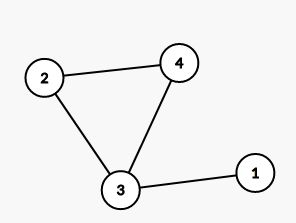
\includegraphics[width=0.3\textwidth]{imgs/graph-stable-set.png}
\end{figure}

Some stable sets are: $\{v_1\}$, $\{v_1, v_2\}$, $\{v_1, v_4\}$, and the
maximum for this graph contains two vertices.

\paragraph{We can model this problem as an ILP}
\begin{equation*}
\begin{aligned}
& \max
& & \sum_{v \in V} x v \\
& \text{st}
& & xv + xw \leq 1, \; \forall \{v, w\} \in E
& & xv \in \{0,1\} \; \forall v \in V
\end{aligned}
\end{equation*}

\paragraph{Proposition: If $G$ is bipartite, then the optimal solution to
$\max \{ \sum_{v \in V} xv \mid xv + xw \leq 1, xv \in [0,1] \}$ is integral.}

\subparagraph{Proof (idea):}
\begin{figure}[!h]
  \label{fig:projection}
  \centering
    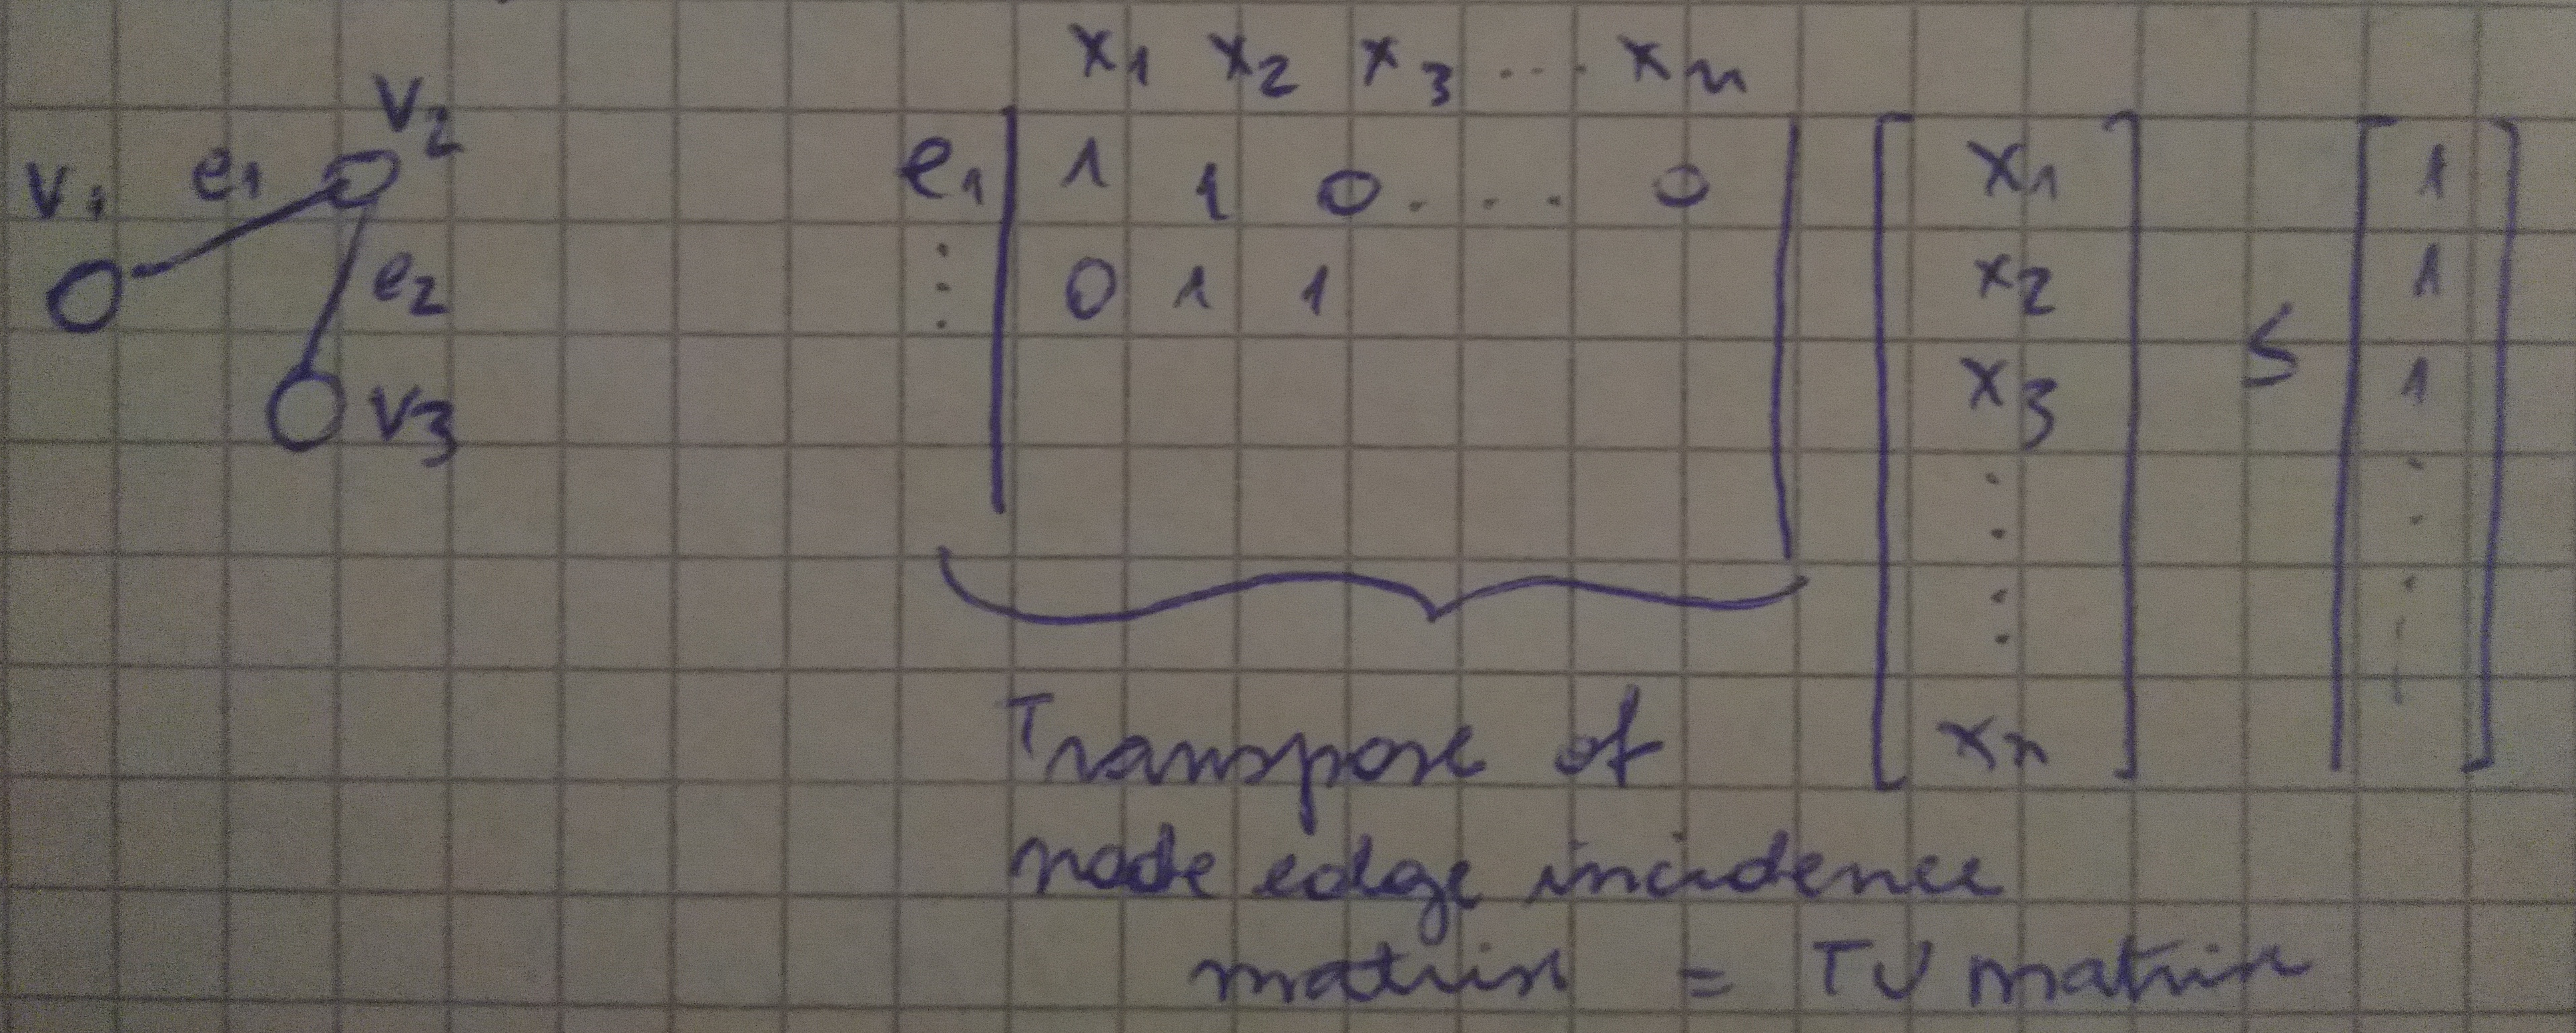
\includegraphics[width=0.6\textwidth]{imgs/bipartite-integral-solution.jpg}
\end{figure}


\paragraph{Definition - (s-t)-flow}
Let $D=(V,A)$ be a digraph. For each $a \in A$, $Ca \in \R_+$ is the \emph{arc 
capacity}. Let $s, t \in V$ with $s \neq t$. A function $x: V \mapsto \R$ is an
\emph{(s-t)-flow} if:
\begin{enumerate}
\item flow conservation constraint: $\sum_{a \in \delta^+(v)} xa = \sum_{a \in
\delta^-(v)} xa$, $\forall v \in V \setminus \{s, t\}$, i.e., the amount of
flow arriving in an intermediate node must be the same amount that comes out.
\item $0 \leq xa \leq Ca$ $\forall a \in A$
\end{enumerate}

The value of $x$ is $val(x) = \sum_{a \in \delta^+(s)} xa - \sum_{a \in
\delta^-(s)} xa$.

\todo[inline]{check figure on notes}

\paragraph{Theorem: If $Ca \in \Z_+$ for all $a \in A$, then the max value of
an (s-t)-flow can be chosen to be integral.}
\subparagraph{Proof:}
Let $M$ be the node-arc incidence matrix of $D$. Define $b \in \R^{|V|}$ as 
$b_i =
\left\{
  \begin{array}{ll}
  0 \text{ if } i \in V \setminus \{s,t\} \\
  ||c||_1 \text{ if } i \in \{s, t\}
  \end{array}
\right.$

A max (s-t)-flow is the solution to $\max \{ \sum_{e \in \delta^+(s)} xe - 
\sum_{e \in \delta^-(s)} xe$ st $-b \leq M \leq b$ and $0 \leq x \leq c\}$

\paragraph{Definition - cut} Let $D=(V,A)$ and $w \subseteq V$. The set
$\delta^+(w)$ is a cut (induced by $w$). An (s-t)-cut satisfies $s \in w$ and
$t \notin w$. Given $c \in \R^{|A|}_+$, the capacity of $\delta^+(w)$ is
$c(\delta^+(w)) = \sum_{a \in \delta^+(w)} Ca$.

\todo[inline]{example on notes}

\paragraph{Lemma: Given $D=(V,A)$ and $s \neq t \in V$, let $x$ be an
(s-t)-flow. For every $w \subseteq V$ st $s \in w$, $t \notin w$, $val(x) =
\sum_{a \in \delta^+(w)} xa - \sum_{a \in \delta^-(w)} xa$.}
Intuitively, $val(x)$ is (flow out of $w$) - (flow into $w$).

\subparagraph{Proof}
proof requires some manipulation of definition
\todo[inline]{prove!}

\paragraph{Lemma: Let $x$ be an (s-t)-flow and $\delta^+(w)$ an (s-t)-cut. Then
$val(x) \leq c(\delta^+(w))$, i.e., the amount of the flow is at most the
amount of the cut.}

\subparagraph{Proof:}
$val(x) = \sum_{a \in \delta^+(w)} xa - \sum_{a \in \delta^-(w)} xa$, each $x$
is bounded by $0$ and $Ca$, then $$val(x) \leq \sum_{a \in \delta^+(w)} Ca -
\sum_{a \in \delta^-(w)} 0 = c(\delta^+(w))$.

\paragraph{Theorem: Let $D=(V,A)$, $s \neq t \in V$, $c \in \R^{|A|}_+$. The
max value of an (s-t)-flow is equal to the min capacity of an (s-t)-cut.}

\subparagraph{Proof:}
The max flow can be solved using:
\begin{equation*}
\begin{aligned}
& \max
& & z\\
& \text{st}
& & x(\delta^-(v)) - x(\delta^+(v)) = 0, \; \forall v \in V \setminus \{s,t\}
& & x(\delta^-(s)) - x(\delta^+(s)) + z = 0
& & x(\delta^-(t)) - x(\delta^+(t)) - \bar{z} = 0
& & xa \leq Ca, \; \forall a \in A
& & xa \geq 0
\end{aligned}
\end{equation*}

The dual LP is 
\begin{equation*}
\begin{aligned}
& \min
& & \sum_{a \in A} Caya\\
& \text{st}
& & ya + zv - zu \geq 0, \; \forall a = (u,v) \in A
& & zs = 0
& & zt = 1
& & ya \geq 0, \; \forall a \in A
\end{aligned}
\end{equation*}

let $x^*$ be an optimal solution to LP (max). From previous lemma, it is enough
to find an (s-t)-cut satisfying $val(x^*) = c(\delta^+(w))$. Let $(y^*, z^*)$
be an optimal dual solution and set $w = \{ u \in V \mid zu^* > 0\}$.\\
If $a=(u,v) \in \delta^+(w)$ then $zu^* > 0$, $zv^* \leq 0$.

$y^* a > 0$. By complementary slackness $x^* a = Ca$ if $a =(u,v) \in \delta^-
(w)$, then $y^*a + zv - zu > 0$, so, $x^*a = 0$. Thus, $val(x) = \sum_{a \in 
\delta^+(w)} xa - \sum_{a \in \delta^-(w)} xa = \sum_{a \in \delta^+(w)} Ca -
\sum_{a \in \delta^-(w)} 0 = c(\delta^+(w))$.


\end{document}
